
%#############################################################################
%
%              						CHAPTER 
%
%#############################################################################
 
\textcolor{cyan}{\chapter{Les bases mathématiques pour le Machine Learning}}
		%{État des connaissances}
	\section{Eléments de calcul différentiel}
	Cette section est inspirée des notes écrites par le Professeur TSHIMANGA \cite[voir][page:45-82]{jtshiman:2021} et d'autres consignes données par Nocedal et al dans \cite{bottou2018optimization} \cite{coulombeau2013math}[??].
	\subsection{Convexité}
		\paragraph*{Définition : (Ensemble convexe)} 
		Une partie $\mathcal{C} \subset \mathbb{R}^n $ est dite convexe si et seulement si pour tout $(x,y) \in \mathcal{C}^2$, 
		et pour tout $ \alpha \in [0, 1]$,
		$ \alpha x + (1 - \alpha)y \in \mathcal{C}$ combinaison convexe \cite{jtshiman:2021}.
		\begin{figure}[bth]
			\centering
			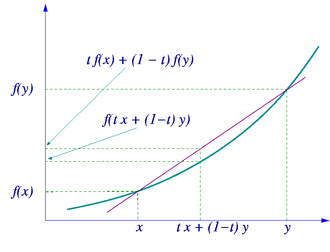
\includegraphics{images/convex_function_graph.png}
			\caption{Illustration fonction convexe [image de Wikipédia]}
			\label{fig:convexe_graph}
		\end{figure}
	
	
	
		
		\paragraph*{Définition : (Fonction convexe)}
		Une fonction $f$ d'un intervalle réel $I \in \mathcal{C}$ est dite fonction convexe lorsque, $\forall (x,y)$ de $I$ tel que $(x,y) \in \mathcal{C}^2$ et tout $\alpha \in [0, 1]$  on a :
		
				
		\begin{equation}
			f(\alpha x + (1 - \alpha)y) \leq \alpha f(x) + (1 - \alpha)f(y)
			\label{eq_convexe-1}
		\end{equation}
		et si
		\begin{equation}
			f(\alpha x + (1 - \alpha)y) < \alpha f(x) + (1 - \alpha)f(y)
			\label{eq_convexe-2}
		\end{equation}
		on dit que la fonction est strictement convexe dans $\mathcal{C}$,  \cite[voir dans][page:45]{jtshiman:2021}\\\\
		Exemple \cite{jtshiman:2021}: 
		\begin{itemize}
			\item[--] La fonction $ f(x) = x^2$ est convexe. 
			\item[--] La fonction $ f(x) = x^T x$ est convexe.
			\item[--] La fonction $ f(x) = x^T Ax$ est convexe, ssi A est symétrique semi-définie positive.
		\end{itemize}
	
		%\subsection{Extrema}	
		\paragraph*{Propriété d'une fonction dérivable : } (Extremum local) 
		Parmi les propriétés de dérivabilité il existe une qui est mise en relation avec l'effect qu'une fonction doit être convexe. énoncé ci-dessous \cite[voir dans][page:212]{coulombeau2013math}.\\
		\begin{list}{+}{Soit $I \rightarrow  \mathbb{R} $ une fonction et $a$ un point de $I$.}
			\item  {On dit que $m$ est un \textbf{minimum local} de $f$ s'il existe $a > 0$ tel que $m$ soit le minimum de $f$ restreinte à $I \cap ] a-\alpha, a + \alpha [$. }
			\item On dit que $M$ est un \textbf{maximum local} de $f$ s'il existe $a > 0$ tel que $M$ soit le maximum de $f$ restreinte à $I \cap ] a-\alpha, a + \alpha [$. 
		\end{list} 
		
		Donc nous pouvons dire qu'une fonction convexe à un unique point minimum.
		
		 
		\subsubsection{Développement limité}\label{sec:dev_lim}
		En physique et en mathématiques, un développement limité (noté DL) d'une fonction en un point est une approximation polynomiale de cette fonction au voisinage de ce point, c'est-à-dire l'écriture de cette fonction sous la forme de la somme d'une fonction polynomiale et d'un reste négligeable au voisinage du point considéré \cite{coulombeau2013math}.
		
		Soit $f$ une fonction à valeurs réelles définie sur un intervalle $I$, et $x_0 \in I$. On dit que $f$ admet un développement limité d'ordre $n^2$ (abrégé par $DL_n$) en $x_0$, s'il existe $n + 1$ réels $a_0, a_1, \dots, a_n$  tels que la fonction ${\displaystyle R:I\to \mathbb {R} }$ définie par :
		$${\displaystyle f(x)=a_{0}+a_{1}(x-x_{0})+a_{2}(x-x_{0})^{2}+\dots+a_{n}(x-x_{0})^{n}+R(x)=\sum _{i=0}^{n}a_{i}(x-x_{0})^{i}+R(x)}$$
		vérifie : $R(x)$ tend vers $0$ lorsque $x$ tend vers $x_0$, et ce plus rapidement que le dernier terme de la somme, c'est-à-dire que :
		$$
			\lim _{{x\rightarrow x_{0}}}{\frac{R(x)}{(x-x_{0})^{n}}}=0. 
		$$
		
		La fonction reste $R(x)$ vérifiant ceci est notée $o((x – x0)^n)$ (selon la notation de Landau). On écrit donc :
		
		$$
			f(x)= \sum _{i=0}^{n}a_{i}(x-x_{0})^{i}+R(x) =\sum _{{i=0}}^{n}a_{i}(x-x_{0})^{i}+o((x-x_{0})^{n})
		$$
		
		%\begin{tabular}{r l}
			%\( f(x)\) & \( =\sum _{i=0}^{n}a_{i}(x-x_{0})^{i}+R(x)\) \\
			%& \(=\sum _{{i=0}}^{n}a_{i}(x-x_{0})^{i}+o((x-x_{0})^{n}) \)
		%\end{tabular}
		
		Il est fréquent d'écrire un développement limité en posant $x = x0 + h$ on aura:
		
		
		$$
			f(x_{0}+h)=\sum _{{i=0}}^{n}a_{i}h^{i}+o(h^{n})
		$$
		
		\paragraph*{Conséquences immédiates}
		\begin{itemize}
			\item Si $f$ admet un $DL_0$ en $x_0$, alors $a_0 = f(x_0)$. \cite{coulombeau2013math}
			\item Si $f$ admet un $DL_n$ en $x_0$, alors elle admet un $DL_k$ en $x_0$ pour tout entier $k < n$ \cite{coulombeau2013math}.
			\item Une condition nécessaire et suffisante pour que f admette un $DL_n$ en $x_0$ est l'existence d'un polynôme $P$ tel que $f(x) = P(x) + o((x – x_0)^n)$ \cite{coulombeau2013math}. S'il existe un tel polynôme $P$, alors il en existe une infinité d'autres, mais un seul d'entre eux est de degré inférieur ou égal à $n$ : le reste de la division euclidienne de $P(X)$ par $(X – x_0)^{n+1}$. On l'appelle la partie régulière, ou partie principale, du $DL_n$ de $f$ en $x_0$. %On identifie parfois, par abus de langage, le $DL_n$ avec sa partie régulière.
		\end{itemize}
		
		
			
		Le théorème de Taylor-Young assure \cite[voir dans][page:241]{coulombeau2013math} qu'une fonction $f$ dérivable n fois au point $x_0$ (avec ${\displaystyle n\geq 1}n\geq 1)$ admet un DLn en ce point :
		
		$$
			{\displaystyle f(x)=f(x_{0})+f'(x_{0})(x-x_{0})+{\frac {f''(x_{0})}{2!}}(x-x_{0})^{2}+\dots +{\frac {f^{(n)}(x_{0})}{n!}}(x-x_{0})^{n}+o((x-x_{0})^{n})}
		$$
		
		soit en écriture abrégée
		$$
			f(x)=\sum _{{i=0}}^{n}{\frac  {f^{{(i)}}(x_{0})}{i!}}(x-x_{0})^{i}+o((x-x_{0})^{n})
		$$
		
		Le développement d'ordre $0$ en $x_0$ revient à écrire que $f$ est continue en $x_0$ :
		
		$$
		{\displaystyle f(x)=f(x_{0})+o((x-x_{0})^{0})=f(x_{0})+o(1)}
		$$
		
		Le développement limité d'ordre 1 en $x_0$ revient à approcher une courbe par sa tangente en $x_0$ on parle aussi d'approximation affine :
		
		$$
		f(x)=f(x_{0})+f'(x_{0})\cdot (x-x_{0})+o(x-x_{0})
		$$
		
		\subsubsection{Différentiabilité au sens de Fréchet} \label{sec:drv_frechet}
			Soient $E$ un espace vectoriel normé, $F$ un espace vectoriel topologique séparé, $f$ une application de $E$ dans $F$ et $a$ un point de $E$. On abandonne la notation des vecteurs par des flèches dans ce paragraphe.
			
			On dit que $f$ est différentiable en $a$ (au sens de Fréchet) s'il existe une application linéaire continue ${\displaystyle L:E\to f}$ telle que :
			$$
			\forall h\in E\quad f(a+h)=f(a)+L(h)+o\left(\|h\|\right)
			$$
			ou, de manière équivalente :
			
			$$
			\lim _{h\to 0}{\frac {f(a+h)-f(a)-L(h)}{\|h\|}}=0.
			$$
			
			Une telle application linéaire $L$ est alors unique.
			L’opérateur $L$ est appelé différentielle de Fréchet (ou F-différentielle, ou Fréchet-différentielle) de $f$ au point $a$, et $f$ est dite Fréchet-différentiable (ou différentiable, ou différentiable au sens de Fréchet) au point $a$. La différentielle de $f$ au point $a$ est souvent notée $Df(a)$, la notation
			$f'(a)$ est aussi utilisée.
	\subsection{Fonctions dérivables}
		
	
	\subsubsection{Gradient}\label{sec:gradient}
		\paragraph*{Définition:}Le gradient d'une fonction de plusieurs variables en un certain point est un vecteur qui caractérise la variabilité de cette fonction au voisinage de ce point. Défini en tout point où la fonction est différentiable, il définit un champ de vecteurs, également dénommé gradient. Le gradient est la généralisation à plusieurs variables de la dérivée d'une fonction d'une seule variable.%\\ \\
		\paragraph*{Définition mathématique :} Dans un système de coordonnées cartésiennes, le gradient d'une fonction {$ f(x_{1},x_{2},\dots ,x_{n}$)} est le vecteur de composantes {$ \partial f/ \partial x_{i}\ (i=1,2,\dots ,n)$}, c'est-à-dire les dérivées partielles de $f$ par rapport aux coordonnées \cite{jtshiman:2021}.
		$${\nabla f(x)={
				\begin{bmatrix}
					{\frac {\partial f(x)}{\partial x_{1}}}\\
					\vdots \\
					{\frac {\partial f(x)}{\partial x_{n}}}
				\end{bmatrix}}} \in \mathbb{R}^n $$
		\pagebreak
		\paragraph*{Gradient sous forme de développement limité:}
		\textit{Si une application admet un gradient en un point, alors on peut écrire ce développement limité du premier ordre (voir le point \ref{sec:dev_lim})}.
		
		$${ 
			f(x+h)=f(x)+\langle \nabla f(x)\mid h\rangle +o(h) 
		}$$ 
		ou 
		$$ {  
			f(x-h)=f(x)-\langle \nabla f(x)\mid h\rangle +o(h)
		}$$
		\textit{Numériquement, il est très intéressant de faire ensuite la demi-différence des deux développements pour obtenir la valeur du gradient et on note que celui-ci ne dépend pas en fait de la valeur de la fonction au point $x : f (x)$. Cette formule a l'avantage de tenir compte des gradients du 2e ordre et est donc beaucoup plus précise et numériquement robuste. L'hypothèse est, en pratique, de connaitre les valeurs "passé" et "futur" de la fonction autour d'un petit voisinage du point $x$}.\\
		\paragraph*{Définition numérique:}
		Une fonction multivariée (à variable vectorielle)
		$ f(x)	: \mathbb{R}^n \rightarrow \mathbb{R} : x \rightarrow f(x) $ définie sur un ouvert $O \in \mathbb{R}^n$ est dite dérivable (au sens de Fréchet, voir le point \ref{sec:drv_frechet}) en $x$ ssi il existe un vecteur noté $\nabla f(x) \in \mathbb{R}^n$ tel que
		\begin{equation}
			f(x+h) = f(x) + \nabla f(x)^{T}h + o(||h||)
		\end{equation}
		
		$\nabla f(x) \in \mathbb{R}^n$ et où l’on a posé que le reste $o(||h||) = ||h||\epsilon (h) \in \mathbb{R}^n$, avec $h \in \mathbb{R}^n$ 
		\begin{center}
			$\epsilon (h): \mathbb{R}^n\rightarrow \mathbb{R}, \hspace{1 cm} \lim\limits_{||h|| \rightarrow 0} \epsilon(h)=0$.
		\end{center} 
		Le vecteur $\nabla f(x)$ est unique et s’appelle \textbf{gradient} de $f(x)$ en $x$.
		Le gradient s’adresse aux fonctions scalaires à variables vectorielles.
		\paragraph*{A propos de la notation $\textbf{o(||h||)}$:}
		La notation de Landau $o(||h||)$ traduit le comportement d’une fonction de $h$ qui [est ??] tend vers $0$ d’un ordre de grandeur plus vite que $||h||$.\\\\
		Elle est infiniment plus petit que $h$ dans le voisinage de $0$
		
		
		
			
	\subsubsection{Hessienne}
	\paragraph*{Définition mathématique:}
	Étant donnée une fonction ${f}$ à valeurs réelles
	
	$${ f:\mathbb{R}^{n}\to \mathbb {R} ;(x_{1},...,x_{n})\mapsto f(x_{1},...,x_{n})}$$
	dont toutes les dérivées partielles secondes existent, le coefficient d'indice ${ i,j}$ de la \textbf{matrice hessienne\footnote{En mathématiques, la matrice hessienne (ou simplement la hessienne) d'une fonction numérique $f$ est la matrice carrée, notée $H(f)$, de ses dérivées partielles secondes.}} ${H(f)}$ vaut ${H_{ij}(f)={\frac {\partial ^{2}f}{\partial x_{i}\partial x_{j}}}}$.\\
	Autrement dit,
	$$
	{ H(f)={
		\begin{bmatrix}{
			\frac {\partial ^{2}f}{{\partial x_{1}}^{2}}}&{\frac {\partial ^{2}f}{\partial x_{1}\partial x_{2}}}&\cdots &{\frac {\partial ^{2}f}{\partial x_{1}\partial x_{n}}}\\
			{\frac {\partial ^{2}f}{\partial x_{2}\partial x_{1}}}&{\frac {\partial ^{2}f}{{\partial x_{2}}^{2}}}&\cdots &{\frac {\partial ^{2}f}{\partial x_{2}\partial x_{n}}}\\
			\vdots &\vdots &\ddots &\vdots \\
			{\frac {\partial ^{2}f}{\partial x_{n}\partial x_{1}}}&{\frac {\partial ^{2}f}{\partial x_{n}\partial x_{2}}}&\cdots &{\frac {\partial ^{2}f}{{\partial x_{n}}^{2}}}
		\end{bmatrix}}} .
	$$
	
	\paragraph*{Définition numérique:}
	Supposons que $f : \mathbb{R}^{n} \to \mathbb{R}$ définie sur un ouvert $\mathcal{O} \in \mathbb{R}^{n}$. La fonction $f(x)$ est dite 2
	fois continûment dérivable (au sens de Fréchet??) si en tout $x \in \mathcal{O}$ on a
	
	\begin{equation}
		f(x + h) = f(x)+\nabla f(x)^Th + \frac{1}{2}h^T\nabla^2f(x)h+o(||h||^2)
	\end{equation}
	avec$\nabla f(x)\in \mathbb{R}^{n\times n}$ et où on a posé que le reste 
	$ o(||h||^2) =||h|| \epsilon(h) \in \mathbb{R} $ avec 
	$\lim\limits_{||h|| \to 0} \epsilon(h) = 0 $
	La matrice carrée symétrique $\nabla^2 f(x)$ appelée \textbf{Hessien} de $f(x)$ en $x$. Remarque :
	
	$$
		\lim\limits_{||h|| \to h} \frac{o(||h||^2)}{||h||} = 0  \in \mathbb{R}
	$$
	La Hessienne s’adresse aux fonctions scalaires à variables vectorielles.
			
	\subsubsection{Jacobienne}
	\paragraph*{Définition mathématique:}
	Soit F une fonction d'un ouvert de $\mathbb{R}^{n}$ à valeurs dans $\mathbb{R}^{m}$ ($F:\mathbb{R}^{n}\to \mathbb {R}^{m}$). Une telle fonction est définie par ses $m$ fonctions composantes à valeurs réelles :
	
	$$ 
	{ F:
		{\begin{pmatrix}
			x_{1}\\\vdots \\
			x_{n}
		\end{pmatrix}}
		\longmapsto 
		{\begin{pmatrix}
			f_{1}(x_{1},\dots ,x_{n})\\
			\vdots \\f_{m}(x_{1},\dots ,x_{n})
		\end{pmatrix}}}.
	$$
	Les dérivées partielles de ces fonctions en un point $M$, si elles existent, peuvent être rangées dans une matrice à $m$ lignes et $n$ colonnes, appelée \textbf{matrice jacobienne\footnote{En analyse vectorielle, la matrice jacobienne est la matrice des dérivées partielles du premier ordre d'une fonction vectorielle en un point donné.}} de $F$ :
	$$
	J_{F}\left(M\right)={
		\begin{pmatrix}
			{\dfrac {\partial f_{1}}{\partial x_{1}}}&\cdots &{\dfrac {\partial f_{1}}{\partial x_{n}}}\\
			\vdots &\ddots &\vdots \\
			{\dfrac {\partial f_{m}}{\partial x_{1}}}&\cdots &{\dfrac {\partial f_{m}}{\partial x_{n}}}
		\end{pmatrix}}.
	$$
	
	La case sur la ligne i et la colonne j contient ${\displaystyle {\frac {\partial f_{i}}{\partial x_{j}}}}$ qui est la dérivée partielle de fi selon la variable xj. Cette matrice est notée :
	
	$${\displaystyle J_{F}\left(M\right),\qquad {\frac {\partial \left(f_{1},\ldots ,f_{m}\right)}{\partial \left(x_{1},\ldots ,x_{n}\right)}}\qquad {\text{ou}}\qquad {\frac {\mathrm {D} \left(f_{1},\ldots ,f_{m}\right)}{\mathrm {D} \left(x_{1},\ldots ,x_{n}\right)}}}$$
	
	Pour $i = 1, … , m,$ la i-ème ligne de cette matrice est la transposée du vecteur \textbf{gradient} (voir le point \ref{sec:gradient}) au point $M$ de la fonction $f_i$, lorsque celui-ci existe. La matrice jacobienne est également la matrice de la différentielle de la fonction, lorsque celle-ci existe.
	\paragraph*{Définition numérique:}
	
	Soit $f(x) : \mathbb{R}^n \to \mathbb{R}^m$ définie sur un ouvert $ \mathcal{O} \subset \mathbb{R} $. On dit que $f(x)$ est dérivable
	(au sens de Fréchet) en $x$, si chacune des composantes $f_i(x)$ est dérivable  en $x$. On a alors
	
	\begin{equation}
		f(x + h) = f(x) + D_f (x)h + o(||h||)
	\end{equation}
	avec $D_f (x) \in  \mathbb{R}^{n \times m} $ et/où $ o(||h||)=||h|| \epsilon(h) \in \mathbb{R}^m $ avec $\lim\limits_{||h|| \to 0} \epsilon(h) = 0 $.
	Remarque :
	$$
		\lim\limits_{||h|| \to h} \frac{o(||h||^2)}{||h||} = 0  \in \mathbb{R}
	$$
	
	Soient 
	$x = 
		\begin{bmatrix}
			x_1 & x_2& \cdots & x_n
		\end{bmatrix}^{T}
		\in \mathbb{R}^n $ et $ 
	f(x) = 
		\begin{bmatrix}
			f_1(x) & f_2(x)& \cdots & f_n(x)
		\end{bmatrix}^{T} \in \mathbb{R}^m
	$
	
	$$
	D_f\left(x\right)={
		\begin{bmatrix}
		{\dfrac {\partial f_{1}(x)}{\partial x_{1}}}&\cdots &{\dfrac {\partial f_{1}(x)}{\partial x_{n}}}\\
		\vdots &\ddots &\vdots \\
		{\dfrac {\partial f_{m}(x)}{\partial x_{1}}}&\cdots &{\dfrac {\partial f_{m}(x)}{\partial x_{n}}}
		\end{bmatrix}}
		=
		\begin{bmatrix}
		\nabla f_1(x)^T \\ \nabla f_2(x)^T\\ \vdots \\ \nabla f_m(x)^T
		\end{bmatrix}
		\in  \mathbb{R}^{n \times m},
	$$
	La matrice $D_f (x) \in  \mathbb{R}^{n \times m} $ est appelée \textbf{Jacobienne} de f(x) en x.
	La Jacobienne s’adresse aux fonctions vectorielles à variables vectorielles.
	
	
	
		
		
	\begin{description}
		\item[Note:] Lorsque $m=1$ (m : nombre des lignes), la Jacobienne est la même que le gradient car il s'agit d'une généralisation du gradient.
	\end{description}
	
		
		
		
	\section{Statistique \& probabilité}

	\subsection{Échantillonnage (Statistique)}
	
	En statistiques, l'échantillonnage est la sélection d'un sous-ensemble (un échantillon statistique ) d'individus au sein d'une population statistique pour estimer les caractéristiques de l'ensemble de la population. 
	
	
	Sur un échantillon, on peut calculer différents paramètres statistiques de position (moyenne, etc.) ou de dispersion (écart type, etc.) issus de la statistique descriptive, de la même manière que l'on peut déterminer des paramètres statistiques d'une population par son recensement exhaustif.
	
	On peut également déduire des propriétés de la population à partir de celles de l'échantillon par inférence statistique. D'après la loi des grands nombres, plus la taille de l'échantillon augmente, plus ses propriétés seront proches de celle de la population. En particulier, on peut estimer une probabilité sur les individus d'une population par la fréquence observée sur un échantillon si sa taille est suffisamment grande. 
	
	Cette méthode présente plusieurs avantages : une étude restreinte sur une partie de la population, un moindre coût, une collecte des données plus rapide que si l'étude avait été réalisé sur l'ensemble de la population, la réalisation de contrôles destructifs, etc.
	
	\begin{list}{$\triangleright$ }{On peut procéder de différentes manières pour collecter les données de l'échantillon, il existe en effet plusieurs méthodes d'échantillonnage \cite{sarndal2003model} :}
		%\textbf
		\item  \textbf{Échantillonnage aléatoire et simple }: le tirage des individus de l'échantillon est aléatoire, c'est-à-dire que chaque individu a la même probabilité d'être choisi, et simple, c'est-à-dire que les choix des différents individus sont réalisés indépendamment les uns des autres.
		%L'échantillonnage aléatoire simple peut être vulnérable aux erreurs d'échantillonnage car le caractère aléatoire de la sélection peut donner un échantillon qui ne reflète pas la composition de la population. 
		
		\item  \textbf{Échantillonnage systématique }: le premier individu est choisi de manière aléatoire, puis les suivants sont déterminés à intervalle régulier. Par exemple, dans un verger, on choisit au hasard le 7e pommier, puis les 27e, 47e, 67e, etc.
		
		\item  \textbf{Échantillonnage stratifié }: on subdivise la population en plusieurs parties avant de prendre l'échantillon1.
		
		\item \textbf{Échantillonnage par quotas }: la composition de l'échantillon doit être représentative de celle de la population selon certains critères jugés particulièrement importants. On utilise cette méthode pour réaliser les sondages d'opinions.
	\end{list}

	
	\subsubsection{La collecte de données }
	
	La collecte de données est le processus de collecte et de mesure des informations sur des variables ciblées dans un système établi, qui permet ensuite de répondre aux questions pertinentes et d'évaluer les résultats.
	
	\begin{list}{--}{Une bonne collecte de données implique :}
		\item Suivre le processus d'échantillonnage défini
		\item Garder les données dans l'ordre du temps
		\item Noter les commentaires et autres événements contextuels
		\item Enregistrement des non-réponses
	\end{list}
	
	\paragraph*{Erreur d'échantillonnage :}
	Dans les statistiques, les erreurs d'échantillonnage se produisent lorsque les caractéristiques statistiques d'une population sont estimées à partir d'un sous-ensemble, ou échantillon, de cette population. Étant donné que l'échantillon n'inclut pas tous les membres de la population, les statistiques de l'échantillon (souvent appelées estimateurs), telles que les moyennes et les quartiles, diffèrent généralement des statistiques de l'ensemble de la population (appelées paramètres ). La différence entre la statistique d'échantillon et le paramètre de population est considérée comme l'erreur d'échantillonnage \cite{sarndal2003model}. 
	
	
	
		
	\subsection{Analyse bayésienne}
		La statistique bayésienne est une théorie dans le domaine des statistiques basée sur l' interprétation bayésienne de la probabilité où la probabilité exprime un degré de croyance en un événement. Le degré de croyance peut être basé sur des connaissances antérieures sur l'événement, telles que les résultats d'expériences précédentes, ou sur des croyances personnelles sur l'événement. Cela diffère d'un certain nombre d'autres interprétations de la probabilité , telles que l' interprétation fréquentiste qui considère la probabilité comme la limite de la fréquence relative d'un événement après de nombreux essais [??].
		
		Les statistiques bayésiennes portent le nom de Thomas Bayes\footnote{Thomas Bayes était un Anglais statisticien , philosophe et ministre presbytérien qui est connu pour la formulation d' un cas spécifique du théorème qui porte son nom : théorème de Bayes.}, qui a formulé un cas spécifique du théorème de Bayes dans un article publié en 1763.
		
		
		
		\begin{thm}[Théorème de Bayes] Le théorème de Bayes est utilisé dans les méthodes bayésiennes pour mettre à jour les probabilités, qui sont des degrés de croyance, après avoir obtenu de nouvelles données. Compte tenu de deux événements $A$  et $B$, la probabilité conditionnelle de $A$ étant donné que $B$ est vrai s'exprime comme suit  :
			\begin{equation}
				\mathbb{P}(A|B) = \frac{\mathbb{P}(B|A) \mathbb{P}(A)}{\mathbb{P}(B)}
			\end{equation}
			
		\end{thm}
	
		où $\mathbb{P}(B) \ne 0$ Bien que le théorème de Bayes soit un résultat fondamental de la théorie des probabilités , il a une interprétation spécifique dans les statistiques bayésiennes \cite[][]{antoine2018apprentissage}.

		
%#############################################################################
%
%              						CHAPTER 
%
%#############################################################################


\textcolor{cyan}{\chapter{Apprentissage automatique : Modélisation et Classification }}
	\section{Généralité}
	\subsection{Les ingrédients d'apprentissage}
	Résoudre un problème d'apprentissage, c'est d'abord le comprendre, c'est-à-dire discuter longuement avec les experts du domaine concerné pour identifier quelles sont les "entrées", les  "sorties" ou résultats désirés, les connaissances disponibles, les particularités des données, par exemple: valeurs manquantes, taux de bruit dans les mesures des attributs de description, proportions des classes, stationnarité ou pas de l'environnement. 
	C'est aussi réaliser un gros travail de \textit{préparation des données}: nettoyage, ré-organisation, enrichissement, intégration avec d'autres sources de données, etc. Ces étapes de compréhension du problème, de préparation des données, de mise au point du protocole d'apprentissage et des mesures d'évaluation des résultats, prennent, et de loin, la plus grande partie du temps pour (tenter de) résoudre un problème d'apprentissage \cite{antoine2018apprentissage}. 
	Nous avons toujours tendance à largement sous-estimer ces étapes et à vouloir se concentrer uniquement sur la phase excitante de l'essai de méthodes d'apprentissage sur des données supposées bonnes à la consommation. 
	\subsubsection{Algorithme qui apprennent}
	
	
	\subsection{Modélisation}\label{sec:modelisation}
	La modélisation est la conception et l'utilisation d'un \textit{modèle}. Selon son objectif et les moyens utilisés, la modélisation est dite mathématique, géométrique, 3D, empirique, etc. 
	En informatique, la modélisation permet de concevoir l'architecture globale d'un système d'information, ainsi que l'organisation des informations à l'aide de la modélisation des données ;
	
	\paragraph*{Modèle (informatique):} En informatique, un modèle a pour objectif de structurer les informations et activités d'une organisation : données, traitements, et flux d'informations entre entités.
	
	\paragraph*{Modèle (mathématique):} Un modèle mathématique est une description d'un système utilisant des concepts et un langage mathématiques.
	
	Un modèle peut aider à expliquer un système et à étudier les effets de différents composants, et à faire des prédictions sur le comportement.
	
	
	\Eg: Prenons l'exemple de données décrites dans l'espace d'entrée $\mathcal{X} = \mathbb{R}^n$ avec $n$ variables réelles et supposons-les étiquetées par $\times$ ou par $\bullet$. On cherche donc une fonction de décision $h$, appelée hypothèse ou modèle, telle qu'elle soit capable d'étiqueter toute entrée 
	$x \in \mathcal{X}, h: x \rightarrow \{\times,\bullet\}$. Reste à définir l'espace des hypothèses ou modèles $\mathcal{H}$ que l'on est prêt à considérer.
	
	Toujours en considérant le problème de prédiction basique (présenté ci-dessus), on pourrait définir une hypothèse par une procédure qui examine les trois plus proches voisins du point à étiqueter $x$ et qui choisit l'étiquette majoritaire parmi ces trois points pour étiqueter $x$. Il n'y a évidemment plus de paramètres pour définir les modèles possibles \cite{antoine2018apprentissage}.
	
	Un \textbf{modèle non paramétrique} est construit selon les informations provenant des données. Dans \cite{antoine2018apprentissage} il est expliqué que : La régression non paramétrique exige des tailles d'échantillons plus importantes que celles de la régression basée sur des modèles paramétriques parce que les données doivent fournir la structure du modèle ainsi que les estimations du modèle
	
	Un \textbf{modèle paramétrique} est, s'il est approximativement valide, plus puissant qu'un modèle non paramétrique, produisant des estimations d'une fonction de régression qui ont tendance à être plus précises que ce que nous donne l'approche non paramétrique \cite{matloff2017statistical}. Cela devrait également se traduire par une prédiction plus précise. 
	
	
	\subsubsection{Entraînement du modèle}
	
	Tout modèle, où toutes les informations nécessaires ne sont pas disponibles, contient certains paramètres qui peuvent être utilisés pour adapter le modèle au système qu'il est censé décrire. Si la modélisation est effectuée par un réseau de neurones artificiels ou un autre apprentissage automatique, l'optimisation des paramètres est appelée \textbf{entraînement} (en anglais : \textbf{training}), tandis que l'optimisation des hyperparamètres du modèle est appelée \textbf{réglage} (en anglais: \textbf{tuning}) et utilise souvent la validation croisée [??]. Dans une modélisation plus conventionnelle à travers des fonctions mathématiques explicitement données, les paramètres sont souvent déterminés par ajustement de courbe.
	
	
	Une partie cruciale du processus de modélisation consiste à évaluer si oui ou non un modèle mathématique donné décrit un système avec précision. Il peut être difficile de répondre à cette question car elle implique plusieurs types d'évaluation différents.
	
	????
	Un modèle de régression linéaire ajusté peut être utilisé pour identifier la relation entre une seule variable prédictive $x_j$ et la variable de réponse $y$ lorsque toutes les autres variables prédictives du modèle sont "maintenues fixes". Plus précisément, l'interprétation de $\beta_j$ est la variation attendue de $y$ pour une variation d'une unité de $x_j$ lorsque les autres covariables sont maintenues fixes, c'est-à-dire la valeur attendue de la dérivée partielle de $y$ par rapport à $x_j$. Ceci est parfois appelé l'effet unique de $x_j$ sur $y$. En revanche, l'effet marginal de $x_j$ sur $y$ peut être évalué à l'aide d'un coefficient de corrélation ou d'un simple modèle de régression linéaire reliant uniquement $x_j$ à $y$; cet effet est la dérivée totale de $y$ par rapport à $x_j$.

	\section{Régression Linéaire}
	Dans la modélisation statistique, l'analyse de régression est un ensemble de processus statistiques permettant d'estimer les relations entre une variable dépendante et une ou plusieurs variables indépendantes [??].\\
	En statistique, la régression linéaire est une approche linéaire pour modéliser (voir le point \ref{sec:modelisation}) la relation entre une réponse scalaire et une ou plusieurs variables explicatives (également appelées variables dépendantes et indépendantes). Le cas d'une variable explicative est appelé régression linéaire simple; pour plus d'un, le processus est appelé régression linéaire multiple.
	
	Dans la régression linéaire, les relations sont modélisées à l'aide de \textit{fonctions prédictives}\footnote{En statistique et en apprentissage automatique, une fonction de prédicteur linéaire est une fonction linéaire d'un ensemble de coefficients et de variables explicatives, dont la valeur est utilisée pour prédire le résultat d'une variable dépendante.} linéaires dont les paramètres de modèle inconnus sont estimés à partir des données \cite{matloff2017statistical}. De tels modèles sont appelés modèles linéaires.
	
	La régression linéaire a de nombreuses utilisations pratiques. Si l'objectif est la prédiction, la prévision ou la réduction des erreurs, la régression linéaire peut être utilisée pour ajuster un modèle prédictif à un ensemble de données observées de valeurs de la réponse et de variables explicatives \cite{darlington2016regression}. Après avoir développé un tel modèle, si des valeurs supplémentaires des variables explicatives sont collectées sans valeur de réponse d'accompagnement, le modèle ajusté peut être utilisé pour faire une prédiction de la réponse.
	
	
	
	
	\subsection{Le problème de la régression linéaire}
		On appelle problèmes de régression de tels problèmes, dans lesquels la sortie est numérique, généralement un vecteur de réels, supposé dépendre de la valeur d'un certain nombre de facteurs en entrée.
		
		Le vecteur d'entrée $x = (1,2,...,x)^T$ est souvent appelé variable indépendante, tandis que le vecteur de sortie $y$ est appelé variable dépendante. On formalise le problème en supposant que la sortie résulte de la somme d'une fonction déterministe $f$ de l'entrée et d'un bruit aléatoire :
		\begin{equation}
			y = f(x) + \epsilon
		\end{equation}
	
		où $f(x)$ est la fonction inconnue que nous souhaitons approcher par un estimateur $h(x|w)$, où $h$ est défini à l'aide d'un vecteur $w$ de paramètres.\\
		Si l'on suppose que le bruit $\epsilon$ est un phénomène gaussien de moyenne nulle et de variance constante $\sigma^2$, c'est-à-dire $ \epsilon = \mathcal{N}(0,\sigma^2)$, alors, en plaçant notre estimateur $h(\cdot)$ à la place de la fonction inconnue, on devrait avoir la densité conditionnelle réelle $p(y|x)$ vérifiant :
		\begin{equation}
			p(y|x) = \mathcal{N}(h(x|w),\sigma^2)
		\end{equation}
		
		On peut estimer le vecteur de paramètres $w$ grâce au principe de maximisation de la vraisemblance. On suppose que les couples $(y_t, y_t)$ de l'échantillon d'apprentissage sont tirés par tirages indépendants d'une distribution de probabilités jointes inconnue $p(x, y)$, qui peut s'écrire :
		
		$$
			p(y|x) = p(y|x)p(x)
		$$
		où $p(y|x)$ est la probabilité de la sortie étant donnée l'entrée et $p(x)$ est la densité de probabilité sur les entrées.
		
		\cite{matloff2017statistical}
		
	%%%\subsubsection*{La régression non linéaire ou multiple}
		%\lipsum[2]
	\subsection{Le cas de la régression générale}
		La plupart des modèles de régression proposent que $Y_{i}$ est une fonction de $X_{i}$ et $\beta$, avec $\epsilon_{i}$ représentant un terme d'erreur additif qui peut remplacer des déterminants non modélisés de $Y_{i}$ ou bruit statistique aléatoire :
		\begin{equation}
			{\displaystyle Y_{i}=f(X_{i},\beta )+\epsilon_{i}}
		\end{equation}
	
	L'objectif est d'estimer la fonction ${\displaystyle f(X_{i},\beta )}$ qui correspond le mieux aux données.
	
	 Pour effectuer une analyse de régression, la forme de la fonction $f$ doit être spécifié. Parfois, la forme de cette fonction est basée sur la connaissance de la relation entre $Y_{i}$ et $X_{i}$. 
	 Si ces connaissances ne sont pas disponibles, un formulaire souple ou pratique pour $f$ est choisi. Par exemple, une simple régression univariée peut proposer
	 $${\displaystyle f(X_{i},\beta )=\beta _{0}+\beta _{1}X_{i}}$$
	 ou
	 $${\displaystyle Y_{i}=\beta _{0}+\beta _{1}X_{i}+e_{i}}$$
	 être une approximation raisonnable du processus statistique générant les données.
	 
	 Différentes formes d'analyse de régression fournissent des outils pour estimer les paramètres. $\beta$. Par exemple, les moindres carrés trouvent la valeur de $\beta$ qui minimise la somme des carrés des erreurs $${\sum _{i}(Y_{i}-f(X_{i},\beta ))^{2}}$$ 
	 
	 Étant donné un ensemble de données ${\displaystyle \{y_{i},\,x_{i1},\ldots ,x_{ip}\}_{i=1}^{n}}$ de $n$ unités statistiques, un modèle de régression linéaire suppose que la relation entre la variable dépendante $y$ et le vecteur $p$ des régresseurs $x$ est linéaire. Cette relation est modélisée par un terme de perturbation ou une variable d'erreur $\epsilon$ : une variable aléatoire non observée qui ajoute du "bruit" à la relation linéaire entre la variable dépendante et les régresseurs. Ainsi le modèle prend la forme
	 
	$${\displaystyle y_{i}=\beta _{0}+\beta _{1}x_{i1}+\cdots +\beta _{p}x_{ip}+\varepsilon _{i}=\mathbf { x} _{i}^{\mathsf {T}}{\boldsymbol {\beta }}+\varepsilon_{i},\qquad avec \quad i=1,\ldots ,n,}
	$$
	
	Souvent, ces $n$ équations sont empilées et écrites en notation matricielle comme
	
	$$
	{\displaystyle \mathbf {y} =X{\boldsymbol {\beta }}+{\boldsymbol {\varepsilon}},\,}
	$$
	
	où
	
	$
	\mathbf{y} ={\begin{pmatrix}y_{1}\\y_{2}\\\vdots \\y_{n}\end{pmatrix}},\quad
	{\displaystyle 
		X={
			\begin{pmatrix}
				\mathbf {x} _{1}^{\mathsf {T}}\\
				\mathbf {x} _{2}^{\mathsf {T}}\\
				\vdots \\
				\mathbf {x} _{n}^{\mathsf {T}}
			\end{pmatrix}}={
			\begin{pmatrix}
				1&x_{11}&\cdots &x_{1p}\\
				1&x_{21} &\cdots &x_{2p}\\
				\vdots &\vdots &\ddots &\vdots \\
				1&x_{n1}&\cdots &x_{np}
			\end{pmatrix}},} \quad
	{\displaystyle {\boldsymbol {\beta }}={
			\begin{pmatrix}
				\beta _{0}\\
				\beta _{1}\\
				\beta _{2}\\
				\vdots \\
				\beta _{p}
			\end{pmatrix}},\quad 
	{\boldsymbol {\varepsilon }}={
		\begin{pmatrix}\varepsilon _{1}\\
			\varepsilon _{2}\\
			\vdots \\
			\varepsilon _{ n}
		\end{pmatrix}}.}$ \\

	$\mathbf{y}$ est un vecteur de valeurs observées ${\displaystyle y_{i}\ (i=1,\ldots ,n)}$ de la variable appelée variable mesurée ou variable dépendante.
	
	$X$ peut être vu comme une matrice de vecteurs-lignes $\mathbf {x} _{i}$ ou de vecteurs-colonnes à $n$ dimensions $X_{j}$, appelées régresseurs, variables explicatives, variables d'entrée, variables prédictives ou variables indépendantes. La matrice $X$ est parfois appelée la matrice de conception. 
	
	${\boldsymbol {\beta}}$ est un vecteur de paramètre de dimension $(p+1)$, où $\beta _{0}$ est le terme d'interception, s'il n'est inclus dans le modèle ${\boldsymbol {\beta}}$ est de dimension $p$. Ses éléments sont appelés effets ou coefficients de régression. 
	En régression linéaire simple , $p = 1$, et le coefficient est appelé \textbf{pente} de régression.\\
	L'estimation statistique et l'inférence dans la régression linéaire se concentrent sur $\beta$. Les éléments de ce vecteur de paramètres sont interprétés comme les dérivées partielles de la variable dépendante par rapport aux différentes variables indépendantes.
		
	%\subsection{La régression linéaire simple}
		%\lipsum[3]
	%\subsection{La régression linéaire multivarié}
		%\subsubsection{Droite de régression} 
		%\subsubsection{Variance, Covariance, \& Corrélation}
	%\subsection{La fonction prédictif \& d'erreur}
		%\lipsum[1]
	
	
	\section{Régression Logistique}
	\subsection{Le problème de classification}
		Lorem ipsum dolor sit amet, consectetur adipiscing elit, sed do eiusmod tempor incididunt ut labore et dolore magna aliqua.
	\subsection{Le cas séparable }
		Lorem ipsum dolor sit amet, consectetur adipiscing elit, sed do eiusmod tempor incididunt ut labore et dolore magna aliqua.
	\subsection{Le cas non séparable }
	
		\begin{figure}
			\centering
			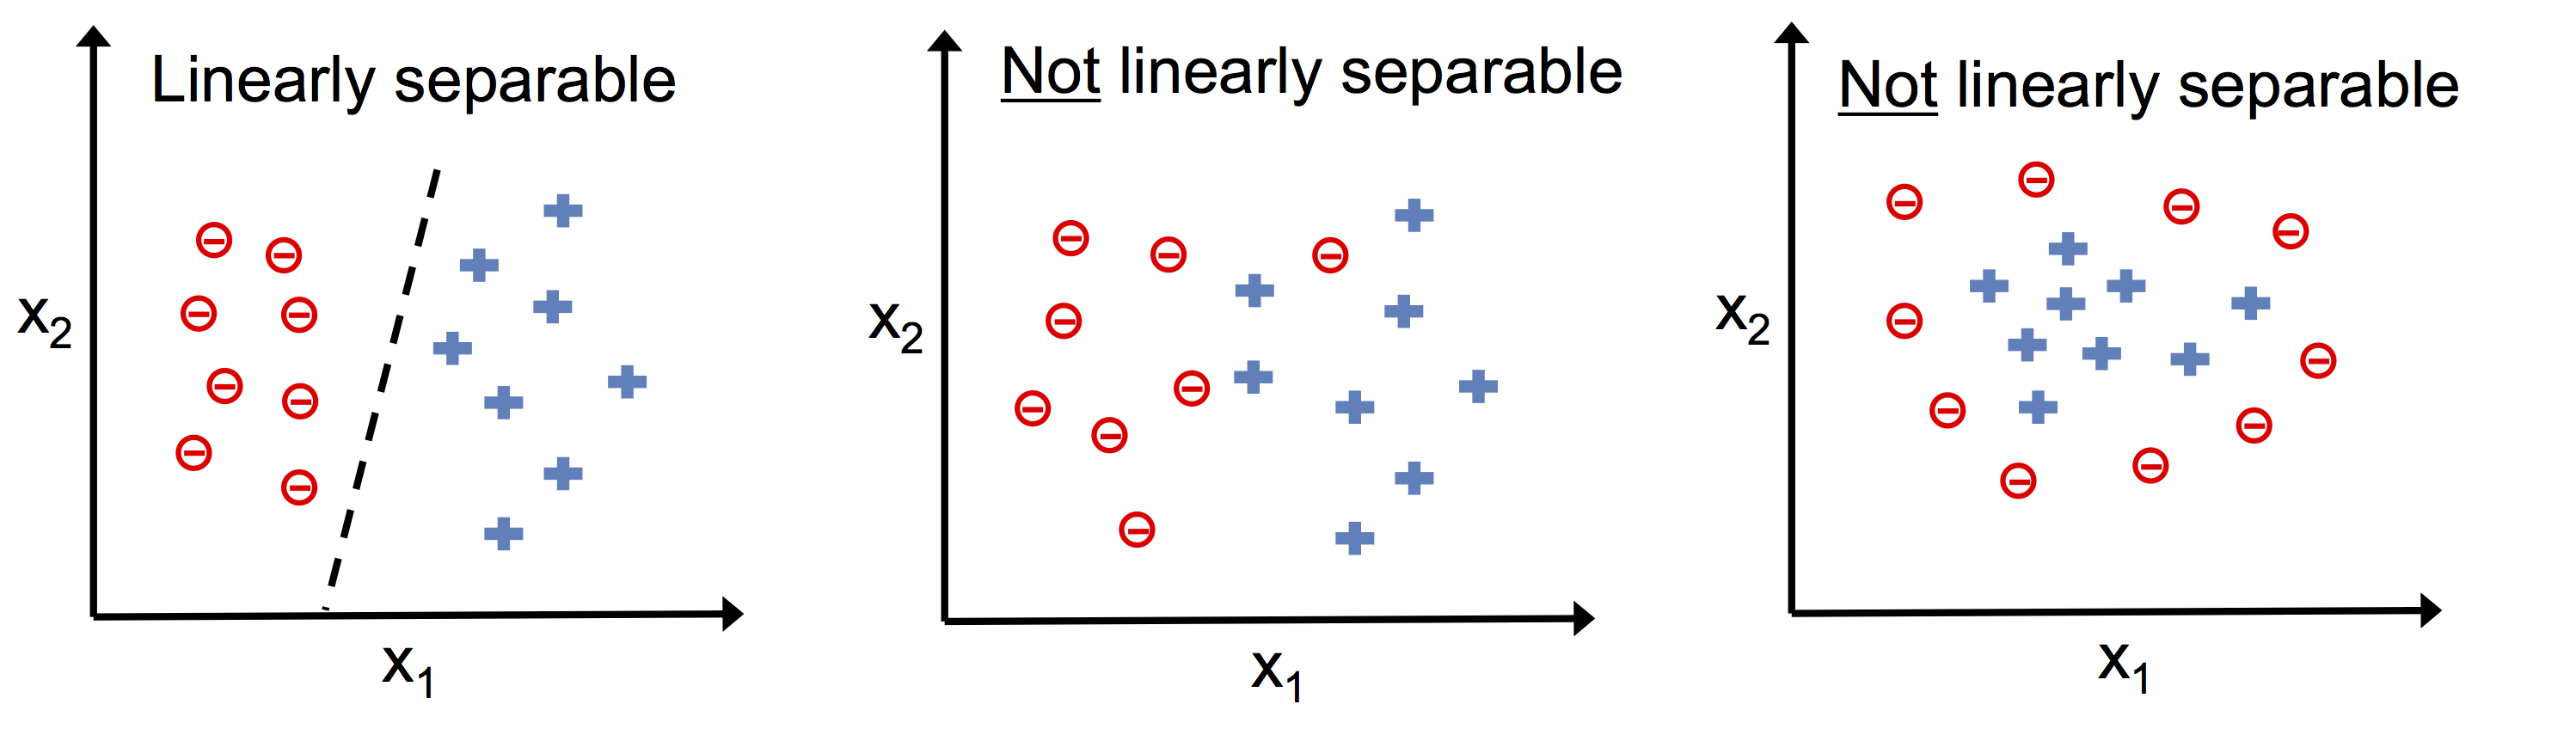
\includegraphics[width=\textwidth]{images/linearly_separable.png}
			\caption{Classes linéairement séparables \cite[image de][page--48]{ml2008python}
		}
			\label{fig:linearly_separable}
		\end{figure}
		\lipsum[3]
	\subsection{Le modèle de la régression logistique }
		\lipsum[1]
		
	\section{Classifications}
	\lipsum[1]
	
	
	\section{Apprentissage profond (Deep Learning)}
	
	\subsection{Perceptron}
	
	\subsection{Neurones}
	\lipsum[1]
	\subsubsection{Réseau neuronal convolutif (CNN)}
	\lipsum[1]
	\subsubsection{Réseau neuronal récurrent (RNN)}
	\lipsum[1]
	
	%\section{Réseaux de neurones}
	
	
	
	%\section{Classificateurs}
	%\lipsum[1]
	

		